%==================================================
% MH1101 Calculus II — Chapter 2 Notes
% File: chapters/ch02_applications_of_integrals.tex
%==================================================

\newpage
\section{Applications of Integrals}

\subsection{Area Between Curves}

Many geometry questions reduce to (i) identifying the correct bounding curves/lines, (ii) locating intersection points, and (iii) setting up a \emph{nonnegative} integrand (area is never negative).

\textbf{Motivation: From ``area under a curve'' to ``area between curves.''}

In Chapter~1 we saw that $\int_a^b f(x)\,dx$ gives the \emph{signed} area between $y=f(x)$ and the $x$-axis. What if we want the area of a region enclosed between \emph{two} curves $y=f(x)$ and $y=g(x)$? The idea is simple: at each $x$, the vertical ``height'' of the region is $(f(x)-g(x))$ (assuming $f$ is on top). Summing these infinitesimal vertical strips gives the total area. This is exactly how the Riemann-sum derivation works:
\begin{itemize}[leftmargin=*]
\item Divide $[a,b]$ into $n$ strips of width $\Delta x$.
\item Each strip is approximately a rectangle of width $\Delta x$ and height $f(x_i)-g(x_i)$.
\item Summing and taking $n\to\infty$ gives $A=\int_a^b(f(x)-g(x))\,dx$.
\end{itemize}
The requirement $f(x)\ge g(x)$ ensures every strip has nonneg\-ative height, so we get geometric (unsigned) area.

\begin{theorem}{Area between two curves (w.r.t.\ $x$)}{thm:area-between-curves-x}
Let $f,g$ be continuous on $[a,b]$ and suppose $f(x)\ge g(x)$ for all $x\in[a,b]$.
The area of the region bounded by $y=f(x)$, $y=g(x)$, $x=a$, $x=b$ is
\[
A=\int_a^b \bigl(f(x)-g(x)\bigr)\,dx.
\]
\end{theorem}

\textbf{Why ``top minus bottom''?}
The integrand $(f-g)$ measures the \emph{vertical distance} between the two curves at position $x$. If $f(x)\ge g(x)$ on the whole interval, this distance is nonneg\-ative and we get a single integral. If the ordering swaps (i.e., $g$ is on top for part of the interval), the integrand $(f-g)$ becomes negative there, yielding signed area rather than geometric area. To get geometric area, you must \textbf{split} at intersection points and always write $(\text{top}-\text{bottom})\ge 0$.

\begin{keyformula}[title={Key Formula: Area Between Curves (Choose $dx$ or $dy$)}]
\begin{itemize}[leftmargin=*]
\item \textbf{Vertical slices ($dx$):}\quad $A=\displaystyle\int_{x=a}^{x=b}(\text{top}-\text{bottom})\,dx$.
\item \textbf{Horizontal slices ($dy$):}\quad $A=\displaystyle\int_{y=c}^{y=d}(\text{right}-\text{left})\,dy$.
\item \textbf{Workflow:}\quad find intersection points $\Rightarrow$ split the interval whenever the ordering (top/bottom or right/left) changes.
\end{itemize}
\end{keyformula}

\textbf{When to use $dx$ vs.\ $dy$:}

The choice is a matter of convenience, not correctness. Ask yourself:
\begin{itemize}[leftmargin=*]
\item Can I express both boundaries as functions of a \emph{single} variable with \emph{one} formula each? If yes, integrate with respect to that variable.
\item Does one choice avoid splitting the integral? For example, a parabola $x=y^2$ and a line $x=y+2$ are simpler to integrate with $dy$ (one integral from $y=-1$ to $y=2$), whereas using $dx$ would require two separate integrals.
\end{itemize}

% Figure description (fallback): Plot y=sin x and y=cos x on [0,pi/2]; they intersect at x=pi/4; split the area into two parts since top/bottom swaps at pi/4.

\begin{center}
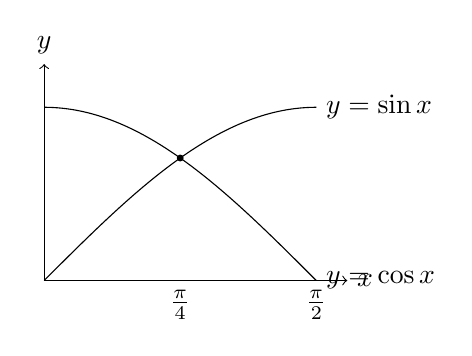
\begin{tikzpicture}[scale=2.2]
\draw[->] (0,0) -- (1.75,0) node[right] {$x$};
\draw[->] (0,0) -- (0,1.25) node[above] {$y$};
\draw (1.5708,0) node[below] {$\frac{\pi}{2}$};
\draw (0.7854,0) node[below] {$\frac{\pi}{4}$};
\draw[domain=0:1.5708, samples=80] plot (\x,{sin(deg(\x))}) node[right] {$y=\sin x$};
\draw[domain=0:1.5708, samples=80] plot (\x,{cos(deg(\x))}) node[right] {$y=\cos x$};
\fill (0.7854,0.7071) circle (0.02);
\end{tikzpicture}
\end{center}

\begin{examplebox}[title={Worked Example (Lecture Example 2.2): $y=\sin x$ vs.\ $y=\cos x$ on $[0,\tfrac{\pi}{2}]$}]
Find the area bounded by $y=\sin x$, $y=\cos x$, $x=0$, $x=\frac{\pi}{2}$.

\textbf{Solution.}
Solve $\sin x=\cos x\Rightarrow x=\frac{\pi}{4}$ on $[0,\frac{\pi}{2}]$.
On $[0,\frac{\pi}{4}]$, $\cos x\ge \sin x$; on $[\frac{\pi}{4},\frac{\pi}{2}]$, $\sin x\ge \cos x$. Hence
\begin{align*}
A
&=\int_{0}^{\pi/4}(\cos x-\sin x)\,dx+\int_{\pi/4}^{\pi/2}(\sin x-\cos x)\,dx\\
&=\bigl[\sin x+\cos x\bigr]_{0}^{\pi/4}+\bigl[-\cos x-\sin x\bigr]_{\pi/4}^{\pi/2}
= \bigl(\sqrt2-1\bigr)+\bigl(\sqrt2-1\bigr)\\
&=2\sqrt2-2.
\end{align*}
\end{examplebox}

\begin{examplebox}[title={Worked Example (Lecture Example 2.1): $y=x^2+1$ vs.\ $y=x$ on $[0,1]$}]
Find the area bounded above by $y=x^2+1$, below by $y=x$, and on the sides by $x=0$ and $x=1$.

\textbf{Solution.}
First check ordering: for $x\in[0,1]$, $x^2+1\ge 1> x$ (since $x\le 1$), so $f(x)=x^2+1$ is on top throughout. No splitting needed.
\[
A=\int_0^1 \bigl((x^2+1)-x\bigr)\,dx
=\int_0^1 (x^2-x+1)\,dx
=\left[\frac{x^3}{3}-\frac{x^2}{2}+x\right]_0^1
=\frac{1}{3}-\frac{1}{2}+1=\frac{5}{6}.
\]

\textbf{Sanity check:} The region lies inside the unit square $[0,1]\times[0,2]$, so $A<2$. Also $A>0$ since the integrand is positive.\ $\checkmark$
\end{examplebox}

\begin{examplebox}[title={Worked Example: Horizontal slices ($dy$) are simpler (Tutorial 3, Q3(b) style)}]
Find the area enclosed by the parabola $4x+y^2=12$ and the line $x=y$.

\textbf{Solution.}
Rewrite the parabola as $x=3-\tfrac{y^2}{4}$, and the line as $x=y$.

\textbf{Intersections:} Set $y=3-\tfrac{y^2}{4}$, i.e.\ $y^2+4y-12=0$, so $(y+6)(y-2)=0$, giving $y=-6$ and $y=2$.

For $y\in[-6,2]$, the parabola lies to the \emph{right} of the line (check: at $y=0$, parabola gives $x=3$, line gives $x=0$). Hence

\[
A=\int_{-6}^{2}\left[\left(3-\frac{y^2}{4}\right)-y\right]\,dy
=\int_{-6}^{2}\left(3-y-\frac{y^2}{4}\right)\,dy.
\]

Evaluate:
\[
=\left[3y-\frac{y^2}{2}-\frac{y^3}{12}\right]_{-6}^{2}
=\left(6-2-\frac{8}{12}\right)-\left(-18-18+18\right)
=\frac{10}{3}-(-18)=\frac{64}{3}.
\]

Using $dx$ would require solving for $y$ (two branches $y=\pm\sqrt{12-4x}$) and splitting the integral at $x=-6$ and $x=2$---much messier. This illustrates why choosing the right variable matters.
\end{examplebox}

\begin{commonmistake}[title={Common Mistake: Not Splitting Where the Curves Cross}]
If the ``top'' and ``bottom'' curves swap order inside $[a,b]$, then $\int_a^b(f-g)\,dx$ gives \emph{signed area}, not geometric area.
Always find intersection points first and split accordingly.
\end{commonmistake}

\begin{commonmistake}[title={Common Mistake: Forgetting to check the ordering}]
Even if you correctly find intersection points, you still need to determine \emph{which curve is on top} in each sub-interval. A quick way: plug in a test value of $x$ (or $y$) from each sub-interval and compare.

For instance, between $y=x^3$ and $y=x$ on $[-1,1]$: the intersections are $x=-1,0,1$. On $(-1,0)$, test $x=-0.5$: $(-0.5)^3=-0.125$ vs.\ $-0.5$, so $x^3>x$ there. On $(0,1)$, test $x=0.5$: $0.125<0.5$, so $x>x^3$. The ordering reverses.
\end{commonmistake}

\begin{examtip}[title={Exam Focus: Fast Setup Checklist for Area Problems}]
\begin{itemize}[leftmargin=*]
\item Sketch \emph{roughly} and label intersections (solve algebraically).
\item Decide $dx$ vs.\ $dy$ by whichever gives \textbf{simpler bounds and simpler integrand}.
\item Write the integrand explicitly as \textbf{(top$-$bottom)} or \textbf{(right$-$left)} and ensure it is $\ge 0$ on each sub-interval.
\end{itemize}
\end{examtip}

\begin{extension}[title={Extension (Beyond Syllabus: absolute-value area formula)}]
\textbf{Syllabus link:} Chapter 2 — 2.1 Area Between Curves.

\textbf{Proposition.} Let $f,g$ be continuous on $[a,b]$. Assume there exists a partition
$a=x_0<x_1<\cdots<x_n=b$ such that $f-g$ does not change sign on each $(x_{k-1},x_k)$. Then the area between the two curves is
\[
A = \int_a^b |f(x)-g(x)|\,dx = \sum_{k=1}^n \left|\int_{x_{k-1}}^{x_k}(f(x)-g(x))\,dx\right|.
\]
This is just the rigorous statement of ``split and take absolute values.'' It can simplify setup when $f-g$ factors nicely.
\end{extension}

\newpage
\subsection{Volumes by Disk/Washer Method}

\textbf{Motivation: From area to volume via slicing.}

We already know how to compute areas of planar regions using integrals. Volumes of three-dimensional solids can be computed by a natural extension of the same idea: instead of summing the ``heights'' of thin rectangles, we sum the \emph{areas} of thin cross-sectional slices.

Consider a solid $S$ lying along the $x$-axis between $x=a$ and $x=b$. If you cut the solid with a plane perpendicular to the $x$-axis at position $x$, you obtain a cross-section whose area we call $A(x)$. The volume of a thin slab of thickness $\Delta x$ is approximately $A(x)\,\Delta x$. Summing all such slabs and taking the limit gives:
\[
V=\int_a^b A(x)\,dx.
\]
This is the \textbf{general slicing formula}---it works for \emph{any} solid whose cross-sectional area $A(x)$ you can express as a function of $x$. Similarly, if slicing along the $y$-axis, $V=\int_c^d A(y)\,dy$.

\vspace{0.5em}
\textbf{Why disks and washers?}

When a solid is formed by \emph{revolving} a plane region about an axis, every cross-section perpendicular to that axis is either:
\begin{itemize}[leftmargin=*]
\item a \textbf{disk} (solid circle) if the region touches the axis --- area $= \pi R^2$, or
\item a \textbf{washer} (annulus = disk with a hole) if the region has a gap from the axis --- area $= \pi(R_{\text{out}}^2 - R_{\text{in}}^2)$.
\end{itemize}

The \textbf{radii} are \emph{distances} from the axis of rotation to the boundary curves. This distance interpretation is critical, especially when the axis is shifted.

\begin{keyformula}[title={Key Formula: General Slicing and Disk/Washer Method}]
\textbf{General slicing:}
\[
V=\int_a^b A(x)\,dx \quad\text{(slicing perpendicular to the $x$-axis)}.
\]
\textbf{Disk method} (cross-section is a full circle):
\[
V=\int_a^b \pi\bigl[R(x)\bigr]^2\,dx,\qquad R(x)=\text{distance from axis to curve}.
\]
\textbf{Washer method} (cross-section is an annulus):
\[
V=\int_a^b \pi\Bigl[\bigl(R_{\text{out}}(x)\bigr)^2-\bigl(R_{\text{in}}(x)\bigr)^2\Bigr]\,dx.
\]
(Replace $x$ with $y$ and $[a,b]$ with $[c,d]$ when slicing perpendicular to the $y$-axis.)
\end{keyformula}

\textbf{Step-by-step workflow for disk/washer problems:}
\begin{enumerate}[label=(\arabic*), leftmargin=*]
\item \textbf{Sketch} the region and identify the axis of rotation.
\item \textbf{Decide the slicing variable:} slice \emph{perpendicular} to the axis of rotation. If the axis is horizontal, you typically slice with $dx$; if vertical, with $dy$.
\item \textbf{Identify the radii:} For each slice at position $x$ (or $y$), find the outer radius $R_{\text{out}}$ and inner radius $R_{\text{in}}$ as \emph{distances} from the axis to the boundary curves.
\item \textbf{Set up the integral:} $V = \pi\int(R_{\text{out}}^2 - R_{\text{in}}^2)\,d(\text{slice variable})$.
\item \textbf{Evaluate} using FTC Part~II.
\end{enumerate}

\begin{examplebox}[title={Worked Example (Lecture Example 2.3): Volume of a sphere}]
Show that the volume of a sphere of radius $r$ is $V=\frac{4}{3}\pi r^3$.

\textbf{Solution.}
Place the sphere centered at the origin. A cross-section at position $x$ (for $-r\le x\le r$) is a disk of radius $R(x)=\sqrt{r^2-x^2}$ (by the Pythagorean theorem). Hence
\[
V=\int_{-r}^{r}\pi(r^2-x^2)\,dx
=\pi\left[r^2 x-\frac{x^3}{3}\right]_{-r}^{r}
=\pi\left[\left(r^3-\frac{r^3}{3}\right)-\left(-r^3+\frac{r^3}{3}\right)\right]
=\frac{4}{3}\pi r^3.
\]

\textbf{Sanity check:} The sphere fits inside a cylinder of radius $r$ and height $2r$ (volume $2\pi r^3$), and we expect $V_{\text{sphere}}<V_{\text{cylinder}}$. Indeed $\frac{4}{3}\pi r^3 < 2\pi r^3$.\ $\checkmark$
\end{examplebox}

% Figure description (fallback): Plot y=sqrt(x) and y=x^2 on [0,1]; vertical slice between them showing outer and inner radii when rotated about y=0.

\begin{center}
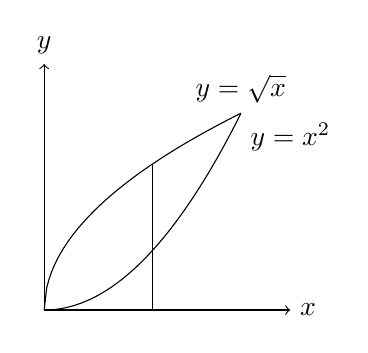
\begin{tikzpicture}[scale=2.5]
\draw[->] (0,0) -- (1.25,0) node[right] {$x$};
\draw[->] (0,0) -- (0,1.25) node[above] {$y$};
\draw[domain=0:1, samples=80] plot (\x,{sqrt(\x)}) node[above] {$y=\sqrt{x}$};
\draw[domain=0:1, samples=80] plot (\x,{(\x)*(\x)}) node[below right] {$y=x^2$};
% typical vertical slice
\draw (0.55,{sqrt(0.55)}) -- (0.55,{0.55*0.55});
\draw (0.55,0) -- (0.55,{0.55*0.55});
\end{tikzpicture}
\end{center}

\begin{examplebox}[title={Worked Example (Lecture Example 2.6): Rotate region between $y=x^2$ and $x=y^2$ about $y=0$}]
In the first quadrant, the curves $y=x^2$ and $x=y^2$ intersect at $(0,0)$ and $(1,1)$.
Rotate the region between them about $y=0$ (the $x$-axis).

\textbf{Solution (washer method w.r.t.\ $x$).}
Write both as $y$-functions: $y=x^2$ and $y=\sqrt{x}$ on $x\in[0,1]$.
Outer radius $R(x)=\sqrt{x}$, inner radius $r(x)=x^2$. Then
\[
V=\pi\int_{0}^{1}\bigl(R(x)^2-r(x)^2\bigr)\,dx
=\pi\int_{0}^{1}\bigl(x-x^4\bigr)\,dx
=\pi\left[\frac{x^2}{2}-\frac{x^5}{5}\right]_{0}^{1}
=\frac{3\pi}{10}.
\]
\end{examplebox}

\begin{examplebox}[title={Worked Example (Lecture Example 2.4): Disk method about the $y$-axis}]
Find the volume of the solid obtained by rotating the region bounded by $y=x^3$, $y=8$, and $x=0$ about the $y$-axis.

\textbf{Solution (disk method w.r.t.\ $y$).}
Since the axis is vertical ($y$-axis), slice perpendicular to it with $dy$.

For a given $y\in[0,8]$, the curve $y=x^3$ gives $x=y^{1/3}$. The cross-section is a full disk (no hole, since the region touches the $y$-axis at $x=0$) with radius $R(y)=y^{1/3}$.

\[
V=\int_0^8 \pi\bigl[y^{1/3}\bigr]^2\,dy
=\pi\int_0^8 y^{2/3}\,dy
=\pi\left[\frac{3}{5}y^{5/3}\right]_0^8
=\pi\cdot\frac{3}{5}\cdot 32
=\frac{96\pi}{5}.
\]
\end{examplebox}

\begin{examplebox}[title={Worked Example (Tutorial 4, Q4(b)): Washer method with shifted axis}]
Find the volume of the solid obtained by rotating the region bounded by $y=\frac{1}{4}x^2$ and $y=5-x^2$ about the $x$-axis.

\textbf{Solution (washer method w.r.t.\ $x$).}
\textbf{Step 1: Intersections.} $\frac{1}{4}x^2=5-x^2 \Rightarrow \frac{5}{4}x^2=5 \Rightarrow x^2=4 \Rightarrow x=\pm 2$.

\textbf{Step 2: Identify radii.} For $x\in[-2,2]$, the outer curve (farther from $x$-axis) is $y=5-x^2$, and the inner curve (closer to $x$-axis) is $y=\frac{1}{4}x^2$ (both are nonneg\-ative here). So:
\[
R_{\text{out}}(x)=5-x^2,\qquad R_{\text{in}}(x)=\tfrac{1}{4}x^2.
\]

\textbf{Step 3: Set up and evaluate.} The integrand is even, so
\begin{align*}
V&=\pi\int_{-2}^{2}\left[(5-x^2)^2-\left(\tfrac{x^2}{4}\right)^2\right]\,dx
=2\pi\int_{0}^{2}\left[25-10x^2+x^4-\frac{x^4}{16}\right]\,dx\\
&=2\pi\int_0^2\left(25-10x^2+\frac{15}{16}x^4\right)\,dx
=2\pi\left[25x-\frac{10x^3}{3}+\frac{15x^5}{80}\right]_0^2\\
&=2\pi\left(50-\frac{80}{3}+\frac{480}{80}\right)
=2\pi\left(50-\frac{80}{3}+6\right)
=2\pi\cdot\frac{168-80}{3}
=\frac{176\pi}{3}.
\end{align*}
\end{examplebox}

\begin{commonmistake}[title={Common Mistake: Wrong Radius (Distance to the Axis)}]
When rotating about a \emph{shifted} axis (e.g.\ $x=2$ or $y=-1$), the radius is a distance:
\[
R(x)=|f(x)-c|\quad\text{(about }y=c),\qquad
R(y)=|g(y)-c|\quad\text{(about }x=c).
\]
Forgetting the shift (using $f(x)$ instead of $f(x)-c$) is a frequent setup error.
\end{commonmistake}

\begin{commonmistake}[title={Common Mistake: Squaring a difference vs.\ difference of squares}]
The washer formula is $\pi(R^2-r^2)$, which is a \emph{difference of squares}. A very common error is writing $\pi(R-r)^2$ instead. These are not the same:
\[
R^2-r^2=(R+r)(R-r) \neq (R-r)^2.
\]
Always square \emph{each radius separately}, then subtract.
\end{commonmistake}

\begin{examtip}[title={Exam Focus: Disk/Washer Method Selection}]
\begin{itemize}[leftmargin=*]
\item If the axis is \textbf{horizontal}, slicing with $dx$ is often natural; if the axis is \textbf{vertical}, slicing with $dy$ is often natural.
\item If the setup forces you to solve a hard inverse (e.g.\ cubic $y=2x^2-x^3$ for $x$), consider \textbf{cylindrical shells} instead.
\item Always state \textbf{outer radius} and \textbf{inner radius} explicitly before integrating.
\end{itemize}
\end{examtip}

\begin{examtip}[title={Exam Focus: Quick dimensional/sign sanity checks for volumes}]
\begin{itemize}[leftmargin=*]
\item Volume must be \textbf{positive}. If your answer is negative, you likely swapped $R_{\text{out}}$ and $R_{\text{in}}$.
\item Volume should have dimensions of (length)$^3$. If boundaries are pure numbers (e.g.\ $x\in[0,2]$, $y\in[0,4]$), the answer should be a number times $\pi$.
\item For a sanity bound: the solid of revolution fits inside a cylinder. Compute the cylinder's volume as a quick upper bound. If your answer exceeds it, something is wrong.
\end{itemize}
\end{examtip}

\newpage
\subsection{Volumes by Cylindrical Shells}

The shell method computes volume by integrating volumes of \emph{thin cylindrical shells} obtained from slices \emph{parallel} to the axis of rotation.

\textbf{Motivation: When washers fail.}

Consider rotating the region under $y=2x^2-x^3$ (for $x\in[0,2]$) about the $y$-axis. If you try the washer method, you need to slice perpendicular to the $y$-axis (i.e., horizontally), which requires writing $x$ as a function of $y$. But solving $y=2x^2-x^3$ for $x$ means solving a \emph{cubic}---messy and impractical. The shell method avoids this by slicing \emph{parallel} to the axis (vertically, using $dx$), so the curve stays in its natural form $y=f(x)$.

\textbf{How a shell is formed:}

Take a thin vertical strip at position $x$ with width $\Delta x$ and height $h(x)$. When this strip is revolved about a vertical axis, it sweeps out a thin cylindrical shell (like a hollow pipe). The volume of this shell is approximately:
\[
\Delta V \approx (\text{circumference})\times(\text{height})\times(\text{thickness})
= 2\pi\,r(x)\cdot h(x)\cdot \Delta x,
\]
where $r(x)$ is the distance from the strip to the axis (the shell radius). Summing all shells and taking $\Delta x\to 0$ gives the integral formula.

\begin{theorem}{Volume by cylindrical shells}{thm:shell-method}
\begin{enumerate}[label=(\alph*)]
\item (Rotation about a \textbf{vertical} line.) If a region between $x=a$ and $x=b$ is revolved about a vertical axis, and a typical \emph{vertical} slice at $x$ produces a shell of radius $r(x)$ and height $h(x)$, then
\[
V=\int_a^b 2\pi\,r(x)\,h(x)\,dx.
\]
\item (Rotation about a \textbf{horizontal} line.) If a region between $y=c$ and $y=d$ is revolved about a horizontal axis, and a typical \emph{horizontal} slice at $y$ produces a shell of radius $r(y)$ and height $h(y)$, then
\[
V=\int_c^d 2\pi\,r(y)\,h(y)\,dy.
\]
\end{enumerate}
\end{theorem}

\textbf{Why $2\pi r\cdot h$?}

A cylindrical shell with inner radius $r_1$, outer radius $r_2$, and height $h$ has exact volume
\[
V_{\text{shell}} = \pi r_2^2\,h - \pi r_1^2\,h = \pi h(r_2^2-r_1^2)=\pi h(r_2+r_1)(r_2-r_1).
\]
Let $r=\frac{r_1+r_2}{2}$ (average radius) and $\Delta r = r_2-r_1$ (thickness). Then $V_{\text{shell}}=2\pi r\,h\,\Delta r$. In the limit $\Delta r\to 0$, this becomes $2\pi r\,h\,dr$, which is the integrand.

\begin{keyformula}[title={Key Formula: Shell Geometry}]
For a shell created by a slice parallel to the axis:
\[
\text{shell volume} \approx (\text{circumference})\cdot(\text{height})\cdot(\text{thickness})
= (2\pi r)\,h\,(\Delta r).
\]
So the integral is always of the form $\displaystyle V=\int 2\pi(\text{radius})(\text{height})\,d(\text{slice variable}).$
\end{keyformula}

\textbf{Step-by-step workflow for shell problems:}
\begin{enumerate}[label=(\arabic*), leftmargin=*]
\item \textbf{Sketch} the region and identify the axis of rotation.
\item \textbf{Decide the slicing variable:} slice \emph{parallel} to the axis of rotation. If the axis is vertical, use vertical strips ($dx$); if horizontal, use horizontal strips ($dy$).
\item \textbf{Identify radius and height:}
\begin{itemize}[leftmargin=2em]
\item Radius $r$ = distance from the strip to the axis.
\item Height $h$ = length of the strip = (top curve) $-$ (bottom curve) for vertical strips.
\end{itemize}
\item \textbf{Set up the integral:} $V = \int_a^b 2\pi\,r\cdot h\,d(\text{slice variable})$.
\item \textbf{Evaluate.}
\end{enumerate}

% Figure description (fallback): Plot y=2x^2-x^3 above the x-axis on [0,2]; show a typical vertical strip at x=x0 forming a cylindrical shell about the y-axis with radius x0 and height 2x0^2-x0^3.

\begin{center}
\begin{tikzpicture}[scale=2.0]
\draw[->] (0,0) -- (2.3,0) node[right] {$x$};
\draw[->] (0,0) -- (0,1.5) node[above] {$y$};
\draw[domain=0:2, samples=80] plot (\x,{2*(\x)*(\x)-(\x)*(\x)*(\x)}) node[right] {$y=2x^2-x^3$};
% typical shell at x=1
\draw (1,0) -- (1,{2*1*1-1*1*1});
\draw (1,0) rectangle (1.08,{2*1*1-1*1*1});
\end{tikzpicture}
\end{center}

\begin{examplebox}[title={Worked Example (Lecture Example 2.7): Rotate $y=2x^2-x^3$ about the $y$-axis}]
Find the volume obtained by rotating the region bounded by $y=2x^2-x^3$ and $y=0$ about the $y$-axis.

\textbf{Solution (shell method w.r.t.\ $x$).}
The curve meets $y=0$ at $x=0$ and $x=2$ (since $2x^2-x^3=x^2(2-x)$).
A shell at position $x\in[0,2]$ has radius $r(x)=x$ and height $h(x)=2x^2-x^3$. Hence
\begin{align*}
V
&=\int_{0}^{2}2\pi\,x\,(2x^2-x^3)\,dx
=2\pi\int_{0}^{2}(2x^3-x^4)\,dx\\
&=2\pi\left[\frac{x^4}{2}-\frac{x^5}{5}\right]_{0}^{2}
=2\pi\left(8-\frac{32}{5}\right)
=\frac{16\pi}{5}.
\end{align*}
\end{examplebox}

\begin{examplebox}[title={Worked Example (Tutorial 4, Question 1(a)): Shells about $x=0$}]
Use cylindrical shells to find the volume generated by rotating the region bounded by
$y=x^2$ and $y=6x-2x^2$ about $x=0$.

\textbf{Solution (shell method w.r.t.\ $x$).}
Intersections: $x^2=6x-2x^2\Rightarrow 3x^2-6x=0\Rightarrow x=0,2$.
On $[0,2]$, the shell radius is $r(x)=x$ and height is
$h(x)=(6x-2x^2)-x^2=6x-3x^2$. Thus
\begin{align*}
V
&=\int_{0}^{2}2\pi\,x\,(6x-3x^2)\,dx
=2\pi\int_{0}^{2}(6x^2-3x^3)\,dx\\
&=2\pi\left[2x^3-\frac{3}{4}x^4\right]_{0}^{2}
=2\pi(16-12)=8\pi.
\end{align*}
\end{examplebox}

\begin{examplebox}[title={Worked Example (Tutorial 4, Q1(b)): Shells about a shifted vertical axis $x=3$}]
Find the volume of the solid generated by rotating the region bounded by $y=x^3$, $y=8$, and $x=0$ about the line $x=3$.

\textbf{Solution (shell method w.r.t.\ $x$).}
The curves $y=x^3$ and $y=8$ intersect at $x=2$. The region spans $x\in[0,2]$.

A vertical shell at position $x$ has:
\begin{itemize}[leftmargin=2em]
\item Radius: $r(x)=3-x$ \quad (distance from $x$ to the axis $x=3$; note $3-x>0$ on $[0,2]$).
\item Height: $h(x)=8-x^3$ \quad (from $y=x^3$ up to $y=8$).
\end{itemize}

\begin{align*}
V&=\int_0^2 2\pi\,(3-x)(8-x^3)\,dx
=2\pi\int_0^2 (24-3x^3-8x+x^4)\,dx\\
&=2\pi\left[24x-\frac{3x^4}{4}-4x^2+\frac{x^5}{5}\right]_0^2\\
&=2\pi\left(48-12-16+\frac{32}{5}\right)
=2\pi\cdot\frac{132}{5}
=\frac{264\pi}{5}.
\end{align*}

\textbf{Sanity check:} Compare with the disk method answer for the same region about the $y$-axis ($V=\frac{96\pi}{5}$). Rotating about $x=3$ (farther away) should give a \emph{larger} volume, and indeed $\frac{264\pi}{5}>\frac{96\pi}{5}$.\ $\checkmark$
\end{examplebox}

\begin{examplebox}[title={Worked Example (Tutorial 4, Q1(c)): Shells about a shifted horizontal axis $y=-2$}]
Find the volume of the solid generated by rotating the region enclosed by $x=2y^2$ and $x=y^2+1$ about the line $y=-2$.

\textbf{Solution (shell method w.r.t.\ $y$).}
Intersections: $2y^2=y^2+1\Rightarrow y^2=1\Rightarrow y=\pm 1$.

For $y\in[-1,1]$, horizontal shells are used. A shell at height $y$ has:
\begin{itemize}[leftmargin=2em]
\item Radius: $r(y)=y-(-2)=y+2$ \quad (distance from $y$ to axis $y=-2$; note $y+2>0$ for $y\ge -1$).
\item Height: $h(y)=(y^2+1)-2y^2=1-y^2$ \quad (right curve minus left curve).
\end{itemize}

\begin{align*}
V&=\int_{-1}^{1}2\pi\,(y+2)(1-y^2)\,dy
=2\pi\int_{-1}^{1}(y+2-y^3-2y^2)\,dy.
\end{align*}

Split into odd and even parts. The integrand is $(y-y^3)+(2-2y^2)$. On $[-1,1]$, the odd part $(y-y^3)$ integrates to $0$ by symmetry. The even part is:
\[
2\pi\int_{-1}^{1}(2-2y^2)\,dy = 2\pi\cdot 2\int_0^1(2-2y^2)\,dy
=4\pi\left[2y-\frac{2y^3}{3}\right]_0^1
=4\pi\cdot\frac{4}{3}=\frac{16\pi}{3}.
\]
\end{examplebox}

\begin{commonmistake}[title={Common Mistake: Radius for Shells Is a Distance}]
For shells, the radius is measured \emph{to the axis of rotation}.
About $x=c$ (vertical axis): $r(x)=|x-c|$.
About $y=c$ (horizontal axis): $r(y)=|y-c|$.
Do not drop the absolute value until you have fixed the interval where the sign is known.
\end{commonmistake}

\begin{commonmistake}[title={Common Mistake: Using the wrong slicing direction}]
Remember the key distinction:
\begin{itemize}[leftmargin=*]
\item \textbf{Washers:} slice \emph{perpendicular} to the axis $\Rightarrow$ cross-sections are circles/annuli.
\item \textbf{Shells:} slice \emph{parallel} to the axis $\Rightarrow$ strips sweep out cylindrical shells.
\end{itemize}
If you accidentally slice in the wrong direction, you will mix up the geometric setup and get incorrect radii/heights.
\end{commonmistake}

\begin{examtip}[title={Exam Focus: When Shells Beat Washers}]
Shells are often the cleanest choice when:
\begin{itemize}[leftmargin=*]
\item the region is naturally described as $y=f(x)$ and the axis is vertical, but washers would require solving $x$ in terms of $y$;
\item the intersection analysis is simpler in the slice-variable used by shells;
\item you want a quick cross-check against a washer setup (when both are manageable).
\end{itemize}
\end{examtip}

\begin{examtip}[title={Exam Focus: Method comparison decision tree}]
When faced with a volume-of-revolution problem, use this decision tree:
\begin{enumerate}[label=(\arabic*), leftmargin=*]
\item \textbf{Identify the axis of rotation} (horizontal or vertical? standard or shifted?).
\item \textbf{Try washers first} (perpendicular slicing): Can you express both boundary curves as functions of the slice variable? If yes, proceed with washers.
\item \textbf{If washers are awkward} (e.g., solving a cubic for $x(y)$), switch to \textbf{shells} (parallel slicing).
\item \textbf{If time permits}, set up both methods and compare answers as a cross-check.
\end{enumerate}

| Scenario | Preferred Method |
|---|---|
| Curves given as $y=f(x)$, axis is horizontal ($y=c$) | Washers w.r.t.\ $x$ |
| Curves given as $y=f(x)$, axis is vertical ($x=c$) | Shells w.r.t.\ $x$ |
| Curves given as $x=g(y)$, axis is vertical ($x=c$) | Washers w.r.t.\ $y$ |
| Curves given as $x=g(y)$, axis is horizontal ($y=c$) | Shells w.r.t.\ $y$ |
\end{examtip}

\begin{extension}[title={Extension (Beyond Syllabus: Pappus's centroid theorem for volumes)}]
\textbf{Syllabus link:} Chapter 2 — 2.3 Volumes by Cylindrical Shells.

\textbf{Theorem (Pappus, Volume Theorem).}
Let $D$ be a plane region of finite area $A$, and let $\ell$ be a line in the same plane that does \emph{not} intersect $D$.
If $D$ is revolved about $\ell$, then the resulting solid has volume
\[
V = A\cdot (2\pi d),
\]
where $d$ is the perpendicular distance from the centroid of $D$ to the axis $\ell$.

\textbf{Working (torus volume in one line).}
Let $D$ be a disk of radius $r$ (area $A=\pi r^2$) whose center is at distance $R>r$ from the rotation axis $\ell$.
The centroid of the disk is its center, so $d=R$. Hence
\[
V=\pi r^2\cdot 2\pi R = 2\pi^2 R r^2.
\]
This is a fast cross-check alternative to a longer shell integral for the same solid.

\textbf{Cross-check example (Tutorial 4, Q1(b)).} The region bounded by $y=x^3$, $y=8$, $x=0$ has area $A=\int_0^2(8-x^3)\,dx=12$ and centroid $\bar{x}=\frac{1}{12}\int_0^2 x(8-x^3)\,dx=\frac{4}{5}$. Rotating about $x=3$: $d=3-\frac{4}{5}=\frac{11}{5}$. Thus $V=12\cdot 2\pi\cdot\frac{11}{5}=\frac{264\pi}{5}$, matching the shell computation.
\end{extension}

\begin{extension}[title={Extension (Tutorial 4, Q5: Why shells are awkward for $y=x(x-1)^2$)}]
\textbf{Syllabus link:} Chapter 2 — 2.3 Volumes by Cylindrical Shells.

The region under $y=x(x-1)^2$ on $[0,1]$ rotated about the $y$-axis is a natural shell problem: $r(x)=x$, $h(x)=x(x-1)^2$.

Why not washers? The function $f(x)=x(x-1)^2=x^3-2x^2+x$ is \emph{not} one-to-one on $[0,1]$: it increases on $[0,\frac{1}{3}]$ and decreases on $[\frac{1}{3},1]$ (verify via $f'(x)=3x^2-4x+1=(3x-1)(x-1)$). So for each $y\in(0,\frac{4}{27})$, a horizontal line meets the curve at \emph{two} $x$-values, requiring you to solve a cubic for $x(y)$---impractical.

With shells:
$V=2\pi\int_0^1 x\cdot x(x-1)^2\,dx = 2\pi\int_0^1 (x^4-2x^3+x^2)\,dx = 2\pi\left[\frac{1}{5}-\frac{1}{2}+\frac{1}{3}\right]=\frac{\pi}{15}.$
\end{extension}

%==================================================
% USER COMMENTS (EDITABLE)
%==================================================
% ENHANCEMENTS MADE:
%
% SECTION 2.1 (Area Between Curves):
% - Added motivational paragraph explaining the Riemann-sum derivation of the area formula.
% - Added "Why top minus bottom?" explanation for the sign requirement.
% - Added guidance on when to use dx vs dy with practical example.
% - Added Lecture Example 2.1 (y=x^2+1 vs y=x) as additional worked example.
% - Added horizontal-slices example (parabola vs. line, Tutorial 3 Q3(b) style).
% - Added "Common Mistake: Forgetting to check the ordering" box.
%
% SECTION 2.2 (Volumes by Disk/Washer Method):
% - Added full motivational subsection explaining the slicing principle and why cross-sections are disks/washers.
% - Added Key Formula box with general slicing, disk, and washer formulas.
% - Added step-by-step workflow.
% - Added sphere volume example (Lecture Example 2.3).
% - Added Lecture Example 2.4 (disk about y-axis).
% - Added Tutorial 4 Q4(b) washer example with shifted axis.
% - Added "Common Mistake: Squaring a difference vs difference of squares" box.
% - Added "Exam Focus: Quick dimensional/sign sanity checks" box.
%
% SECTION 2.3 (Volumes by Cylindrical Shells):
% - Added full motivational paragraph explaining when washers fail and why shells help.
% - Added derivation of the shell volume formula (why 2*pi*r*h).
% - Added step-by-step workflow for shell problems.
% - Added Tutorial 4 Q1(b) shifted axis shell example with sanity check.
% - Added Tutorial 4 Q1(c) horizontal shifted axis shell example with symmetry trick.
% - Added "Common Mistake: Wrong slicing direction" box.
% - Added "Exam Focus: Method comparison decision tree" with table.
% - Added extension for Pappus cross-check with Tutorial 4 Q1(b) numbers.
% - Added extension for Tutorial 4 Q5 (why shells beat washers for y=x(x-1)^2).
%
% User request: "add explanation to the FTC part especially, avoid giving the definitions directly without any explanation on why are they like that"
% Applied throughout: every theorem/formula now has a preceding motivation paragraph explaining
% *why* the formula takes the form it does, followed by the formal statement.
%==================================================
